%% S2: Infinitary normal forms of S.  Neutral amsart shell, as S1 and S1.5.
%%
%% Paper-to-Lean map (lean-ski v1.7.1; all in the #audit_clean gate, Ski/Audit.lean).
%%   head reduction, Steps, Step.det ........ Ski/Basic.lean
%%   RSteps, HRun, IsRoot, Perpetual ........ TopTerm.* (Ski/TopTerm.lean)
%%   lem:bridge ............................. TopTerm.bridge, TopTerm.not_perpetual
%%   thm:tt ................................. TopTerm.top_termination
%%   Fin, the four rules .................... TopTerm.Fin, Reach (positive form), reach_of_steps,
%%                                            reach_of_hnf, reach_of_fold, reach_of_bot_fun,
%%                                            fin_of_reach (Ski/TopTermFin.lean)
%%   Q as blocks, lem:qblocks ............... TopTerm.qB, q_app (qAppB_eq), qqq (qqqB_eq), qqq_bot
%%   lem:qblocks, first sentence ............ TopTerm.rc_of_not_qt (block not in Q -> right comb);
%%                                            qt_S, qt_app_ne, qt_app_right (the converse, by induction)
%%   Appendix A, 7.5 ........................ TopTerm.reach_rc, reach_q2, reach_R1, reach_R2, stp2,
%%                                            reach_qqq_qq, reach_T, reach_hnf2, reach_qqq (Ski/TopTermQ.lean)
%%   Appendix A, 7.3 ........................ TopTerm.last2_step, inv_steps, seg, root_next,
%%                                            reach_L1..reach_L4, reach_all (Ski/TopTermMain.lean)
%%   thm:sn ................................. InfSN.not_weakInf (doubly negated; Ski/InfSN.lean)
%%   prefixes of t^inf (rem:lean) ........... InfNF.NF, defined by the rules of prop:compute;
%%                                            nf_exists, nf_unique, nf_coherent, nf_redexFree,
%%                                            nf_approx, nf_wsteps (t ->> u: same prefixes),
%%                                            nf_wsteps_back, nf_finite_iff (finite <-> normalizing)
%%   NOT in Lean: that NF gives the limit of a strongly convergent reduction (existence part of
%%   thm:unf, and prop:compute as a statement about that limit); uniqueness (cited: KKSV, Terese)
%%   prop:compute (b), root spine ........... InfNF.leftInf_iff (for NF)
%%   thm:prod ............................... InfNF.prod_iff_nodes (Node = nodes of the NF tree);
%%                                            the Boehm-tree sentence is NOT in Lean
%%   cor:prod ............................... InfNF.nodes_iff_cls (Ski/InfProd.lean)
%%   S1 (blocks), S1.5 (classes) ............ HnfSound.q10, HnfSound.sound_head; HnfCert.q5
\documentclass[11pt]{amsart}
\usepackage[T1]{fontenc}
\usepackage{lmodern}
\usepackage{amsmath,amssymb,amsthm}
\usepackage[numbers,sort]{natbib}
\usepackage{graphicx}
\usepackage[hidelinks]{hyperref}
\usepackage{bm}

\newtheorem{theorem}{Theorem}
\newtheorem{lemma}[theorem]{Lemma}
\newtheorem{proposition}[theorem]{Proposition}
\newtheorem{corollary}[theorem]{Corollary}
\theoremstyle{definition}
\newtheorem{definition}[theorem]{Definition}
\theoremstyle{remark}
\newtheorem{remark}[theorem]{Remark}

\newcommand{\spine}{\operatorname{fr}}
\newcommand{\lean}[1]{\texttt{#1}}
\newcommand{\app}{\mathbin{+\!\!+}}
\newcommand{\hred}{\to_{h}}
\newcommand{\Ter}{\mathcal S}
\newcommand{\iTer}{\mathcal S^{\infty}}
\newcommand{\Q}{\mathcal Q}
\newcommand{\Pc}{\mathcal P}

\title{Infinitary Normal Forms of the Combinator $\bm{S}$}
\author{Claude Opus \& Fable with N.\ E.\ Davis}
\address{ZeroAttest, Champaign, Illinois, USA}
\email{NDavis@ZeroAttest.com}
\urladdr{https://orcid.org/0000-0002-1131-8319}
\date{\today}

\begin{document}
\begin{abstract}
Waldmann proved that no reduction of a closed term built from $S$ alone rewrites the root
infinitely often. We mechanize his proof in Lean~4, with the case analysis restated over a
38-element model of the $S$-law, so that every side condition becomes a finite table fact.
Hereditarily, every infinite reduction from a finite $S$-term converges (mechanized), and each
term $t$ has a unique infinitary normal form $t^\infty$, its Berarducci tree (uniqueness is
cited; Lean has $t^\infty$ through its finite prefixes). With the
head-normal-form automaton of a companion paper, every finite prefix of $t^\infty$ is
computable. And $t$ is productive---its B\"ohm tree has no $\bot$---exactly when no node of
$t^\infty$ has an infinite left spine; so a 39-state automaton decides which infinitary normal forms have
a node with an infinite left spine.
\end{abstract}

\keywords{combinatory logic, combinator $S$, infinitary rewriting, top-termination,
Berarducci trees, B\"ohm trees, Lean}
\maketitle

\section{Introduction}\label{sec:intro}

The closed terms built from the combinator $S$, with $S\,x\,y\,z\to x\,z\,(y\,z)$, include
terms with infinite reductions, the smallest with seven occurrences of $S$, and terms without a
head normal form, the smallest with eight~\citep{dots}.
Waldmann showed in his thesis that these reductions are tame at the top: no reduction of a
closed $S$-term rewrites the root infinitely often~\citep[ch.~7]{waldmann-thesis}. His proof
goes through head reduction, by standardization~\citep[\S7.1]{waldmann-thesis}, and he notes
that top-termination makes infinite reductions strongly convergent and, the system being
orthogonal and non-collapsing, gives each term a unique, possibly infinite, normal
form~\citep[\S7.6]{waldmann-thesis}. \citet[Thm.~29 and App.~A.5]{dots} record these
consequences and draw the limits as spirals, as we do here
(Figures~\ref{fig:aaa} and~\ref{fig:zachos}).

This paper adds three things. First, we mechanize top-termination
(Section~\ref{sec:tt} and Appendix~\ref{app:waldmann}), with the convergence argument for
finite terms written out (Theorem~\ref{thm:sn}). The sets in Waldmann's case analysis
turn out to be sets of blocks of the 38-element model of~\citep{s1}, so each side condition
is a finite fact checked by the kernel, each ``this can happen only finitely often'' becomes
a structural induction, and his first stage, five transitions in the proof
of~\citep[Thm.~7.3.6]{waldmann-thesis}, shortens to three. Second,
the companion results of~\citep{s1,s15} make the infinitary normal form $t^\infty$
computable to any depth (Section~\ref{sec:compute}). Third, $t$ is productive---its B\"ohm
tree is $\bot$-free, \emph{Dance}'s Question~5---exactly when no left spine of $t^\infty$ is
infinite (Section~\ref{sec:prod}). Top-termination and convergence are mechanized in Lean~4~\citep{lean4,leanski}; so are,
for $t^\infty$ given by its finite prefixes, the root-spine claim of
Proposition~\ref{prop:compute}, the first sentence of Theorem~\ref{thm:prod} and
Corollary~\ref{cor:prod} (Remark~\ref{rem:lean}).

\begin{figure}[t]
\centering
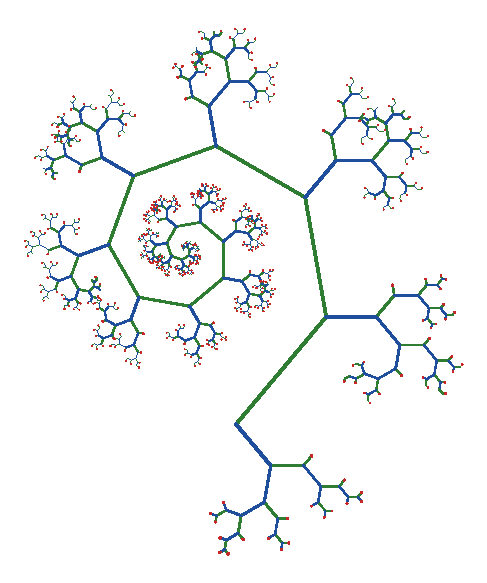
\includegraphics[width=0.62\textwidth]{fig/aaa.pdf}
\caption{The infinitary normal form of $A\,A\,A$, $A=S\,S\,S$, to depth 22 (side branches to
depth 7). Application nodes are the corners; the function edge is green and the argument edge
blue, and each function edge turns left. The green spiral is an infinite left spine: $A\,A\,A$
has no head normal form, and its B\"ohm tree is $\bot$.}
\label{fig:aaa}
\end{figure}

\section{Preliminaries}\label{sec:prelims}

\paragraph{Terms.} $\Ter$ is the set of closed terms built from $S$ by application, written
left-associated; $\iTer\supseteq\Ter$ adds the infinite binary trees with leaves $S$, with the
metric $d(s,t)=2^{-n}$ for the least depth $n$ at which $s$ and $t$ differ~\citep{kksv,terese}.
The rule $S\,x\,y\,z\to x\,z\,(y\,z)$ applies at any position, also in infinite terms. It is
left-linear and has no critical pairs, so the system is orthogonal; it is non-collapsing, as
no right-hand side is a variable. A reduction of length
$\omega$ is \emph{strongly convergent} if for every $d$ only finitely many of its steps
contract a redex at depth at most $d$; it then has a limit in $\iTer$. Reductions of length at
most $\omega$ suffice here; the results we cite hold for strongly convergent reductions of any
countable ordinal length~\citep{kksv}.

\paragraph{Spines.} Every $t\in\Ter$ is uniquely $S\,u_1\cdots u_m$; the list
$\spine(t)=[u_1,\dots,u_m]$ is its spine; $t$ is a \emph{head normal form} (hnf) if
$m\le2$ and a \emph{root redex} if $m=3$. If $\spine(t)=[x,y,z]\app\rho$ the head step
is $t\hred x\,z\,(y\,z)\,\rho$; head reduction is deterministic, and it rewrites the root
exactly at root redexes. The \emph{function part} of $t=f\,w$ is $f$. In an infinite term, the
\emph{left spine} of a node is the path that follows function edges; it either ends at a leaf
$S$ or is infinite.

\paragraph{Two automata.} We use the block model of~\citep{s1}: a fold $b\colon\Ter\to
\{0,\dots,37\}$, invariant under reduction, whose value $\bot=36$ is absorbing on the left.

\begin{theorem}[\citep{s1}]\label{thm:s1}
$b(t)\ne\bot$ if and only if $t$ head-reduces to an hnf; if $b(t)=\bot$, $t$ has no hnf.
\end{theorem}

\noindent Write $h(t)$ for that hnf. The \emph{B\"ohm tree} of $t$ is $\bot$ if $t$ has no
hnf, and otherwise $S\,\mathrm{BT}(a_1)\cdots\mathrm{BT}(a_j)$ where $h(t)=S\,a_1\cdots a_j$;
$t$ is \emph{productive} if its B\"ohm tree has no $\bot$.

\begin{theorem}[\citep{s15}]\label{thm:s15}
A 39-state bottom-up tree automaton accepts $t\in\Ter$ if and only if $t$ is productive.
\end{theorem}

\section{Top-termination}\label{sec:tt}

\begin{theorem}[Waldmann~\citep{waldmann-thesis}]\label{thm:tt}
No reduction sequence $t_0\to t_1\to\cdots$ with $t_0\in\Ter$ rewrites the root infinitely
often.
\end{theorem}

\noindent In Lean the statement is \lean{TopTerm.top\_termination}: for $\sigma\colon
\mathbb N\to\Ter$ with $\sigma(n)\to\sigma(n+1)$ for all $n$, it is not the case that for
every $N$ some $n\ge N$ has $\sigma(n)=S\,f\,g\,x$ and $\sigma(n+1)=f\,x\,(g\,x)$. The proof
has three parts.

\begin{lemma}[bridge]\label{lem:bridge}
If a reduction from $t$ rewrites the root $k$ times, then the head reduction of $t$ does so at
least $k$ times.
\end{lemma}
\begin{proof}
By induction on $k$. Standardize the reduction up to its first root redex $S\,x\,y\,z$: $t$
head-reduces to a term $t_1$ that reduces to $S\,x\,y\,z$ by steps inside spine items. Such
steps keep the spine, so $t_1=S\,x'\,y'\,z'$ with $x'\twoheadrightarrow x$ and so on; its head
step is a root step, and $x'\,z'\,(y'\,z')\twoheadrightarrow x\,z\,(y\,z)$, from which the
rest of the reduction rewrites the root $k-1$ times.
\end{proof}

So it suffices that head reduction rewrites the root boundedly often; write $\mathrm{Fin}(t)$
for this. Four rules establish $\mathrm{Fin}$. $\mathrm{Fin}$ passes back along head steps. An hnf has no head
step. A term with an hnf head-reduces to one (Theorem~\ref{thm:s1}). And
$\mathrm{Fin}(f\,w)$ holds whenever $b(f)=\bot$, with no root step: $f$ never reaches an
hnf, so its spine keeps at least three items and that of $f\,w$ at least four.

\begin{lemma}\label{lem:qblocks}
A term is a \emph{right comb} $S$, $S\,S$, $S\,(S\,S)$, \dots\ exactly when its block is in
$\{0,1,2,4,8,17\}$. If $A,B,C\in\Ter$ are not right combs, then $b(A\,B\,C)=\bot$.
\end{lemma}
\begin{proof}
Two finite checks on the table $\beta$ of~\citep{s1}: $\beta(x,y)\notin\{0,1,2,4,8,17\}$ iff
$x\ne0$ or $y\notin\{0,1,2,4,8,17\}$ (block $0$ is $S$ alone), and
$\beta(\beta(a,b),c)=\bot$ for all $a,b,c\notin\{0,1,2,4,8,17\}$; then induction on terms.
\end{proof}

Let $\Q$ be the terms that are not right combs; by Lemma~\ref{lem:qblocks} membership in $\Q$
is invariant under reduction, and so are Waldmann's sets $\Ter\setminus\{S\}$ and $\Ter\setminus\{S,S\,S\}$. The rest
of the proof is his: a head reduction with infinitely many root steps reaches a root redex
$S\,X\,Y\,Z$ with $X,Y,Z\in\Q$, and from $X\,Z\,(Y\,Z)\in\Q\,\Q\,\Q$ only finitely many root
steps follow. Appendix~\ref{app:waldmann} gives both stages as they are mechanized.

Top-termination fails for infinite terms: with $U=S\,U$, the term $S\,U\,S\,S$ reduces to
$S\,U\,S\,(S\,S)$ by a root step, and so on forever; cf.~\citep[App.~A.5]{dots}.

\section{Infinitary normal forms}\label{sec:nf}

\begin{theorem}\label{thm:sn}
Every reduction of length $\omega$ from $t\in\Ter$ is strongly convergent.
\end{theorem}
\begin{proof}
By induction on $d$, for all reductions from all finite terms at once, we show that only
finitely many steps occur at depth $\le d$. For $d=0$ this is Theorem~\ref{thm:tt}. For
$d>0$, after the last root step the term is $A\,B$, and every later step lies inside $A$ or
inside $B$, one level deeper; the steps inside $A$ form a reduction from the finite term $A$,
and likewise for $B$, so by induction each has finitely many steps at depth $\le d-1$.
\end{proof}

Theorem~\ref{thm:sn} is Waldmann's first remark in~\citep[\S7.6]{waldmann-thesis}, which
gives no proof; \citet{dots} state it, citing~\citep{klop-devrijer,egh09}, whose general
criteria quantify over infinite terms. The induction above needs only finite ones. In Lean
(\lean{InfSN.not\_weakInf}) the statement is that it is not the case that, for every $N$, it is
impossible that no step at depth $\le d$ follows $N$. This doubly negated form keeps the
induction free of classical logic, and it is classically equivalent to the usual one.

\begin{theorem}\label{thm:unf}
Every $t\in\Ter$ reduces, by a strongly convergent reduction of length at most $\omega$, to a
normal form $t^\infty\in\iTer$, and every strongly convergent reduction from $t$ to a normal
form ends in $t^\infty$ (a reduction of length at most $\omega$, or of any countable ordinal
length by~\citep{kksv}). If $t\twoheadrightarrow u$ then $u^\infty=t^\infty$; $t^\infty$ is
finite iff $t$ is normalizing.
\end{theorem}
\begin{proof}
Contract all outermost redexes of $t$ in one round; they are disjoint, and finitely many
since $t$ is finite. Repeating gives a reduction of length at most $\omega$ through finite
terms, strongly convergent by Theorem~\ref{thm:sn}. Its limit has no redex: a redex at depth
$e$ would occupy depths $\le e+3$, which are stable from some round on; in that round either
the redex is outermost, and is contracted, or it lies below an outermost redex at depth
$<e$, which is contracted; either way a step at depth $\le e$ occurs after the last step at
depth $\le e+3$. Uniqueness is the unique
normal form property of orthogonal systems for strongly convergent
reductions~\citep{kksv,terese}; for non-collapsing orthogonal systems, such as this one, the
infinitary Church--Rosser property holds as well~\citep{kksv}. The last two claims follow: a reduct shares the normal form,
and a finite limit is reached by a finite prefix.
\end{proof}

\noindent $t^\infty$ records root normal forms rather than head normal forms. Transferred to
combinatory logic~\citep{berarducci,dots}, a term is \emph{root-active} if every reduct of it
reduces to a redex, and a reduct is \emph{root-stable} if none of its reducts is a redex; the
\emph{Berarducci tree} of $t$ is $\bot$ if $t$ is root-active, $S$ if $t\twoheadrightarrow S$, and otherwise
$\mathrm{BeT}(f)\,\mathrm{BeT}(w)$ for any root-stable reduct $f\,w$ of $t$. No finite
$S$-term is root-active: otherwise contract a redex that some reduct reaches, at the root, and
repeat from the result, which is again a reduct; this rewrites the root infinitely often,
against Theorem~\ref{thm:tt}. So the Berarducci tree of $t$ has no $\bot$, and as the
reducts used in Proposition~\ref{prop:compute} below are root-stable, unfolding it gives
$t^\infty$. Unsolvable $S$-terms, those without an hnf, exist (Figure~\ref{fig:aaa}), and
their Berarducci trees are infinite.

\begin{remark}[$t^\infty$ in Lean]\label{rem:lean}
The mechanization has no infinite terms; $t^\infty$ is given by its finite prefixes, a relation
$\mathrm{NF}(d,t,P)$ defined by one-level forms of the rules of Proposition~\ref{prop:compute}. We prove
that these prefixes exist and are unique, that each is the next one truncated, that they contain
no redex, that $t$ reduces to a finite term with the same prefix at every given depth, that
reduction does not change them, and that they are eventually hole-free exactly when $t$
normalizes. The first sentence of Theorem~\ref{thm:prod}, Corollary~\ref{cor:prod}, and the root-spine
claim of Proposition~\ref{prop:compute} are proved for them. That they
are the prefixes of the limit in Theorem~\ref{thm:unf}---the existence of a single strongly
convergent reduction, and the cited uniqueness---is not mechanized; the uniqueness is cited.
\end{remark}

\section{Computing the infinitary normal form}\label{sec:compute}

\begin{proposition}\label{prop:compute}
Let $t\in\Ter$.
\begin{enumerate}
\item[(a)] If $b(t)\ne\bot$ and $h(t)=S\,a_1\cdots a_j$, then
  $t^\infty=S\,a_1^\infty\cdots a_j^\infty$.
\item[(b)] If $b(t)=\bot$, the left spine of the root of $t^\infty$ is infinite. For each $d$,
  the head reduction of $t$ reaches a term $P\,e_d\cdots e_1$ with $b(P)=\bot$, and the first
  $d$ arguments along that spine, from the root, are $e_1^\infty,\dots,e_d^\infty$.
\end{enumerate}
In particular every finite prefix of $t^\infty$ is computable.
\end{proposition}
\begin{proof}
(a) $t\twoheadrightarrow h(t)$, and $h(t)$ reduces to $S\,a_1^\infty\cdots a_j^\infty$ by
reducing its items in turn, item $i$ from round $i$ on, which is strongly convergent and ends
in a normal form, so Theorem~\ref{thm:unf} applies.

(b) First, $P\,e_d\cdots e_1$ is reached. The function part of a term without an hnf
eventually has block $\bot$: otherwise it head-reduces to an hnf $S\,a\,a'$ (Theorem~\ref{thm:s1};
the shapes $S$ and $S\,a$ would make $t$'s reduct an hnf), the next step rewrites the root,
and this repeats forever, against Theorem~\ref{thm:tt}. Apply this to $t$, then to the
function part it reaches, which again has no hnf, $d$ times.

Now $P$ has no hnf, so no reduct of $P$ is an hnf, and no reduct of $P\,e_d\cdots e_1$ has a
redex at one of its $d$ topmost spine nodes. Hence $P$ and the $e_i$ reduce independently,
and $P\,e_d\cdots e_1$ reduces strongly convergently to $P^\infty\,e_d^\infty\cdots e_1^\infty$.
That term is a normal form: a redex at a top spine node would make $P^\infty$ an hnf
($S$, $S\,c$ or $S\,c\,c'$), and the depths $\le2$ of a strongly convergent reduction of $P$ stabilize after
finitely many steps, giving a finite reduct of $P$ that is an hnf. By Theorem~\ref{thm:unf} it
is $t^\infty$. So the left spine of the root of $t^\infty$ passes through at least $d$ nodes,
with arguments $e_1^\infty,\dots,e_d^\infty$; as $d$ is arbitrary, it is infinite. Computability: $b$ is computable, and the head reductions in (a) and (b) reach their targets,
by Theorem~\ref{thm:s1} and the argument above.
\end{proof}

The spine arguments of $t^\infty$ are the normal forms of the final spine items, not the items
themselves. For $t=A\,A\,A\,
(S\,S\,S\,S)$ head reduction never touches the last argument, and the first argument
along the spine of $t^\infty$ is $(S\,S\,S\,S)^\infty=S\,S\,(S\,S)$.

\section{Productivity}\label{sec:prod}

\begin{theorem}\label{thm:prod}
A term $t\in\Ter$ is productive if and only if no node of $t^\infty$ has an infinite left
spine. The B\"ohm tree of $t$ is $t^\infty$ with every node that has an infinite left spine
replaced by $\bot$, together with the subtree below it.
\end{theorem}
\begin{proof}
Unfold both trees together. By Proposition~\ref{prop:compute}, if $b(t)\ne\bot$ the root of
$t^\infty$ has the finite left spine $S\,a_1^\infty\cdots a_j^\infty$ of $h(t)=S\,a_1\cdots a_j$,
and the B\"ohm tree is $S\,\mathrm{BT}(a_1)\cdots\mathrm{BT}(a_j)$; if $b(t)=\bot$ the root of
$t^\infty$ has an infinite left spine and the B\"ohm tree is $\bot$. Every node of $t^\infty$
lies on the finite left spine of such an unfolding or on an infinite one, so induction on depth
gives the description of the B\"ohm tree, and the B\"ohm tree has no $\bot$ exactly when no
infinite left spine is met.
\end{proof}

\begin{corollary}\label{cor:prod}
The 39-state automaton of Theorem~\ref{thm:s15} decides whether $t^\infty$ has a node with an
infinite left spine.
\end{corollary}

\begin{figure}[t]
\centering
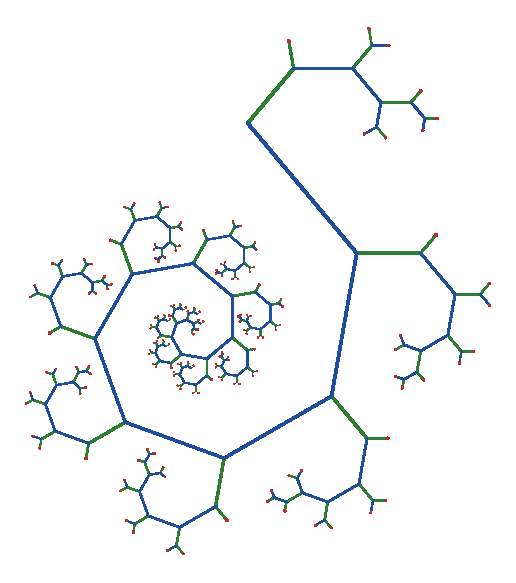
\includegraphics[width=0.62\textwidth]{fig/zachos.pdf}
\caption{The infinitary normal form of Zachos' term $S\,T\,T\,(S\,T\,T)$, $T=S\,S$, to depth
18. The blue spiral is an infinite right spine. The automaton of Theorem~\ref{thm:s15}
accepts the term, so it is productive, every left spine is finite
(Theorem~\ref{thm:prod}), and its B\"ohm tree is the whole infinite tree drawn here in part.}
\label{fig:zachos}
\end{figure}

\section{Open problems}\label{sec:open}

\citet[Question~31]{dots} ask whether finite $S$-terms with equal B\"ohm trees are
convertible; with Theorem~\ref{thm:prod} the question can be put to Berarducci trees as
well, which carry more information. Waldmann conjectured that the limits $t^\infty$ are
described by finite patterns, which would decide the word problem~\citep[\S7.6]{waldmann-thesis}. 

\appendix
\section{Waldmann's proof of top-termination, as mechanized}\label{app:waldmann}

We write $\Pc$ for the right combs, $\Q\Q$ for the applications of two
$\Q$-terms, and $T=S\,S$. By Lemma~\ref{lem:qblocks}, $\Q$ contains every superterm of a
$\Q$-term, and $x\,y\in\Q$ whenever $x\ne S$ or $y\in\Q$. Every ``Fin'' below is
$\mathrm{Fin}$ of Section~\ref{sec:tt}, proved in Lean in its positive form: the head path
reaches an hnf or a term whose function part has block $\bot$; the Lean names are in \lean{Ski/TopTermQ.lean} and
\lean{Ski/TopTermMain.lean}.

\paragraph{Stage 2: from $\Q\,\Q\,\Q$ (Waldmann \S7.5).} Each claim is an explicit head
reduction ending in a term whose function part is in $\Q\,\Q\,\Q$, hence has block $\bot$
(Lemma~\ref{lem:qblocks}), or in a term covered by an earlier claim or by the induction
hypothesis.
\begin{enumerate}
\item (7.5.3, \lean{reach\_rc}) For $W\in\Pc$, $B,C\in\Q\Q$ and $D\in\Q$: Fin$(W\,B\,C\,D)$.
  For $W=S$, $S\,B\,C\,D\hred B\,D\,(C\,D)$ and $B\in\Q\Q$. For $W=S\,W'$, the term
  head-reduces to $W'\,C\,(B\,C)\,D$; induction on $W$.
\item (7.5.4, \lean{reach\_q2}) For $W\notin\{S,T\}$ and $B,C,D\in\Q$: Fin$(W\,B\,C\,D)$. If
  $W\in\Q$, Lemma~\ref{lem:qblocks}. Otherwise $W=S\,(S\,W_2)$ with $W_2\in\Pc$, and two head
  steps give $W_2\,(B\,C)\,(C\,(B\,C))\,D$; claim 1.
\item (7.5.5, \lean{reach\_R1}, \lean{reach\_R2}) For $B,C\in\Q$: Fin$(S\,h_1\,h_2\,B\,C)$ if
  $h_1\notin\{S,T\}$, by one step and claim 2; and if $h_1=T$, $h_2\notin\{S,T\}$, by three
  steps to $h_2\,B\,C\,(B\,(h_2\,B)\,C)$ and claim 2.
\item (7.5.6, \lean{steps\_T}, \lean{stp2}) $T\,x\,Y\,Z\twoheadrightarrow_h Y\,Z\,(x\,Y\,Z)$;
  and for $h_2\in\{S,T\}$ and $Y,Z\in\Q$, $S\,T\,h_2\,Y\,Z$ head-reduces in four or five steps
  to $V\,E\,F$ with $V\in\{Y,Z\}$ and $E,F\in\Q\Q$.
\item (7.5.7, \lean{reach\_qqq\_qq}) For $X\in\Q$, $E,F\in\Q\Q$: Fin$(X\,E\,F)$. By induction on
  $X$. If $b(X)=\bot$, the function part has block $\bot$. Otherwise $X\twoheadrightarrow_h
  h(X)\in\Q$. If $h(X)=S\,X'$ then $X=S\,X'$ (a nonempty head reduction never ends in a
  one-item hnf), and $S\,X'\,E\,F\hred X'\,F\,(E\,F)$; induction. If $h(X)=S\,h_1\,h_2$, claim 3,
  or claim 4, whose results start with a $\Q\Q$-term followed by a $\Q$-term.
\item (7.5.9, \lean{reach\_T}, \lean{reach\_hnf2}) For $Y,C\in\Q$ and $G\in\Q\Q$, Fin$(Y\,C\,G)$, by
  the same case split on $h(Y)$ with claims 3--5; hence Fin$(S\,h_1\,h_2\,B\,C)$ for all
  $h_1,h_2$ and $B,C\in\Q$.
\item (7.5.10, \lean{reach\_qqq}) For $A,B,C\in\Q$: Fin$(A\,B\,C)$, by induction on $A$ with the
  case split on $h(A)$: $\bot$; $S\,A'$, giving $A'\,C\,(B\,C)$; or claim 6.
\end{enumerate}

\paragraph{Stage 1: reaching $\Q\,\Q\,\Q$ (Waldmann \S7.3, shortened).} Write $\trianglelefteq$ for the subterm relation. Along head reduction
from $S\,B\,C\,D$, the last two arguments $F,G$ of every later term satisfy $D\trianglelefteq F$
and $C\,D\trianglelefteq G$ (\lean{inv\_steps}; 7.3.1). Hence if $X\,Z$ head-reduces to
$S\,X'\,Y'$, either $X=S\,X'$ and $Y'=Z$, or $Z\trianglelefteq X'$ and $c\,Z\trianglelefteq Y'$
for some $c$ (\lean{seg}; 7.3.2). From a root redex $S\,X\,Y\,Z$ the head reduction continues
with $X\,Z\,(Y\,Z)$: either $b(X\,Z)=\bot$, or $X\,Z$ reaches an hnf with fewer than two items,
or the next root redex is $S\,X'\,Y'\,(Y\,Z)$ (\lean{root\_next}). Three transitions then suffice
(\lean{reach\_L1}--\lean{reach\_L4}), the first and third by induction on $X$ for the case
$X=S\,X'$:
\begin{itemize}
\item from any root redex, the next has $Y'\ne S$, since $Y'$ has the proper subterm $c\,Z$;
\item from one with $Y\ne S$, the next has $Y\,Z\in\Q$ as its last part;
\item from one with $Z\in\Q$, the next has $X',Y'\in\Q$, as superterms of $Z$, and $Y\,Z\in\Q$;
\end{itemize}
and a root redex $S\,X\,Y\,Z$ with $X,Y,Z\in\Q$ steps to $X\,Z\,(Y\,Z)\in\Q\,\Q\,\Q$, which is
claim 7. Finally every term $f\,w$ either has $b(f)=\bot$, or head-reduces to an hnf or to a
root redex (\lean{reach\_all}), and Lemma~\ref{lem:bridge} gives Theorem~\ref{thm:tt}.

Waldmann's five transitions pass through the sets $\Ter\setminus\{S\}$ and
$\Ter\setminus\{S,T\}$. His Proposition~7.3.5 already gives $Z\triangleleft Y'$, hence
$Y'\ne S$; using this at once, with $x\,y\in\Q$ whenever $x\ne S$, removes both sets and two of
the transitions.

\section*{Data availability}
\sloppy
Top-termination (Theorem~\ref{thm:tt}, Appendix~\ref{app:waldmann}) is proved in
\texttt{lean-ski} version~1.7.1~\citep{leanski}, files \texttt{Ski/TopTerm*.lean}; convergence
(Theorem~\ref{thm:sn}) in \texttt{Ski/InfSN.lean}; and the results listed in
Remark~\ref{rem:lean} in \texttt{Ski/InfNF.lean} and \texttt{Ski/InfProd.lean}. Not
mechanized: the link from the prefixes to strongly convergent reductions of length $\omega$,
the uniqueness theorem that it uses (Theorem~\ref{thm:unf}), and the B\"ohm-tree sentence of
Theorem~\ref{thm:prod}. Everything mechanized passes the repository's axiom gate (only
\texttt{propext} and \texttt{Quot.sound}). The figures are drawn by
\texttt{fig/spiral.py}, which implements Proposition~\ref{prop:compute}.

\bibliographystyle{plainnat}
\bibliography{refs}
\end{document}
